\documentclass[12pt, a4paper, openany, bibliography=totoc]{report} %, BCOR0mm scrbook

% scrartcl ist eine abgeleitete Artikel-Klasse im Koma-Skript
% bibliography=totoc: Literaturverzeichnis im Inhaltsverzeichnis
% zur Kontrolle des Umbruchs Klassenoption draft verwenden
%BCOR: Bindekorrektur


% die folgenden Packete erlauben den Gebrauch von Umlauten und ß
% in der Latex Datei
\usepackage[utf8]{inputenc}
% \usepackage[latin1]{inputenc} %  Alternativ unter Windows
\usepackage[T1]{fontenc}
\usepackage[ngerman]{babel}


\usepackage[paper=a4paper,left=25mm,right=25mm,top=25mm,bottom=25mm]{geometry}
\usepackage[pdftex]{graphicx}
\usepackage{subfigure}
\usepackage{latexsym}
\usepackage{amsmath,amssymb,amsthm}
\usepackage[export]{adjustbox}
\usepackage{pdfpages}
% deutsches Literaturverzeichnis
\usepackage[numbers,round]{natbib}

%neue Seite für jedes Kapitel
%\usepackage{titlesec}
%\newcommand{\sectionbreak}{\clearpage}

% Umgebungen für Definitionen, Sätze, usw.
% Es werden Sätze, Definitionen etc innerhalb eines Chapters mit
% 1.1, 1.2 etc durchnummeriert, ebenso die Gleichungen mit (1.1), (1.2) ..
\newtheorem{Satz}{Satz}[chapter]
\newtheorem{Lemma}[Satz]{Lemma}
\newtheorem{Korollar}[Satz]{Korollar}

\theoremstyle{definition}	
\newtheorem{Definition}[Satz]{Definition}
\newtheorem{Beispiel}[Satz]{Beispiel}
\newtheorem{Bemerkung}[Satz]{Bemerkung}
                    
\numberwithin{equation}{chapter} 

% einige Abkuerzungen
\newcommand{\C}{\mathbb{C}} % komplexe
\newcommand{\K}{\mathbb{K}} % komplexe
\newcommand{\R}{\mathbb{R}} % reelle
\newcommand{\Q}{\mathbb{Q}} % rationale
\newcommand{\Z}{\mathbb{Z}} % ganze
\newcommand{\N}{\mathbb{N}} % natuerliche
\DeclareMathOperator{\sign}{sign}



\begin{document}
  % Keine Seitenzahlen im Vorspann
  \pagestyle{empty}
\begin{titlepage}
	
	\newcommand{\HRule}{\rule{\linewidth}{0.5mm}} % Defines a new command for the horizontal lines, change thickness here
	
	\center % Center everything on the page
	
	%----------------------------------------------------------------------------------------
	%	HEADING SECTIONS
	%----------------------------------------------------------------------------------------
	\hspace*{5.0cm}\\[4cm]

	\textsc{\LARGE Mathematical Aspects\\[0.2cm] of Machine Learning}\\[0.5cm] % Major heading such as course name
	\textsc{\large Report}\\[2cm] % Minor heading such as course title
	
	%----------------------------------------------------------------------------------------
	%	TITLE SECTION
	%----------------------------------------------------------------------------------------
	
	\HRule \\[0.8cm]
	{ \huge \bfseries Digit Recognition\\ with Support Vector Machine}\\[0.8cm] % Title of your document
	\HRule \\[1.5cm]
	
	%----------------------------------------------------------------------------------------
	%	AUTHOR SECTION
	%----------------------------------------------------------------------------------------
	
	\begin{minipage}{0.4\textwidth}
		\begin{flushleft} \large
			\emph{Authors:}\\
			Lisa \textsc{Gaedke-Merzhäuser} \\% Your name
			Paul \textsc{Korsmeier}\\
			Lisa \textsc{Mattrisch}\\
			Vanessa \textsc{Schreck}\\
		\end{flushleft}
	\end{minipage}
	~
	\begin{minipage}{0.4\textwidth}
		\begin{flushright} \large
			\emph{} \\
			 \textsc{} % Supervisor's Name
		\end{flushright}
	\end{minipage}\\[2cm]

	
	
\end{titlepage}

\cleardoublepage
  % Ab sofort Seitenzahlen unten mittig
  \pagestyle{plain}

\chapter*{Problem Statement}
Our main goal is to correctly identify handwritten digits based on the MNIST  ("Modified National Institute of Standards and Technology") data set.
This data set consists of 42000 gray-scale images. Each image is 28 pixels in height and 28 pixels in width. Each pixel has a single pixel-value associated with it, indicating the lightness or darkness of that pixel \cite{kaggel}.

\begin{figure}[h]
	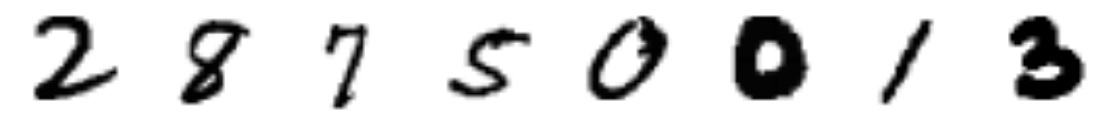
\includegraphics[width=1\textwidth, center]{Digits2}
	\caption{Visualization of eight of these images}
\end{figure}




\chapter*{Support Vector Machine}
Given data points $\{x_i\}_{i=1}^l \subset \R^d$ with labels $\{y_i\}_{i=1}^l \subset \{\pm 1\}$ we want to seperate the different labels using a decision function of the form
$$f(x) = \sign\left(w^T\Phi(x) + b\right)$$ where $\Phi$ is the feature map as introduced in the lecture.
The Support Vector Machine (SVM) is a binary classifier that aims to find the maximum margin hyperplane in the feature space, i.e. the goal is to maximize the margin while softly penalizing points that lie on the wrong side of the boundary or inside the margin \cite{Bishop2006}. After the  dualization of this optimization problem we obtain the following equivalent quadratic program:
\begin{equation*}
\begin{aligned}
& \underset{0 \leq \alpha \leq C}{\text{maximize}}
& & \sum_{i = 1}^{l}\alpha_i - \frac{1}{2} \sum_{i, j = 1}^{l}\alpha_i  \alpha_j y_i y_j k(x_i, x_j)
\end{aligned}
\end{equation*}
with the dual variable $\alpha$, kernel function $k$ and penalty $C$.
After finding the optimal solution $\alpha^*$ of this program we can formulate the decision function as
$$f(x) = \sign\left(\sum_{i=1}^{l}\alpha^*_i y_i k(x_i,x_j)+b\right).$$
Note that only data points $x_i$ with $\alpha_i \neq 0$ appear in the decision funcion. Those points are called \textit{support vectors}. By analysing primal, dual and the corresponding KKT conditions we find that any $x_i$ with $\alpha_i = C$ lies exactly on the margin and any $x_i$ with $0<\alpha_i < C$ lies either inside the margin or on the wrong side of the margin. Additionally any data point $x_i$ on the margin must satisfy $y_i*f(x_i) = 1$. We can use this property to find the parameter $b$ \cite{Bishop2006}.






\chapter*{Solving the optimization problem with SMO}


\chapter*{Multi Class Classification Problem}

Support Vector Machines are binary classifiers, meaning that there only two possible output labels. Usually one chooses them to be $1$ and $-1$. Our problem however was to classify unknown data into one out of $10$ different categories. Since there is no way to change one support vector machine so that it can choose from more than two labels we had to find a way to combine several SVMs, who together would be able to do so. There are a number of well known strategies tackling this issue. Let us first look at two very intuitive but also primitive strategies. The first one is One-vs-All classification. In this approach one trains as many SVMs as one has classes, so 10 in our case, and sets labels so that the i-th SVM has all training data with label i set to one and everything else to $-1$. .... This approach has many issues. Not uniquely classified. Advantage low compute time, one has to at least expect to train $10$ binary classifiers to divide into $10$ different categories. depends on which one first...? some areas several labels...  

The other possibility is called One-vs-One classification. Here one only ever considers the data corresponding to two classes and sets one label to $1$ and the other one to $-1$. ... 
In our case this would mean training $45$ SVMs (the number arises from the binary coefficient of 10 choose 2...). advantage/disadvantage

We only tried the first approach since as just mentioned the compute time for the second one was simply too high for us considering that we have a very large amount of training data. In the One-vs-All results were very very disappointing. In the case of a linear as well as a Gaussian kernel ... In the linear case this can be explained by the fact that our training data was simply not linearly seperable. 
Hence we added in an additional feature. We computed the barycenters of the data points of each class. When a data point could not be uniquely classified we would give it the label of the barycenter it was closest to. This method led to a major improvement of our results. Our algorithm now labeled about 60\% of our data correctly (... see appendix).  Nevertheless the result was still not satisfactory. 

So we decided to focus our attention on a different approach: Error Correcting Output Codes. 
\\
subheading? \\
\\
They are easiest to explain considering a concrete example. We trained 15 different classifiers $f_i$. 

\begin{table}[ht!]
	\centering
	\caption{Error Correcting Output Codes}
	\label{Codewords}
	\begin{tabular}{|l|l|l|l|l|l|l|l|l|l|l|l|l|l|l|l|}
	\hline
	Class	& $f_0$ & $f_1$ & $f_2$ & $f_3$ & $f_4$ & $f_5$ & $f_6$ & $f_7$ & $f_8$ & $f_9$ & $f_{10}$ & $f_{11}$ & $f_{12}$ & $f_{13}$ & $f_{14}$ \\ \hline \hline
	0	& 1 & 1 & -1 & -1 & -1 & -1 & 1 & -1 & 1 & -1 & -1 & 1 & 1 & -1 & 1 \\ \hline
	1	&  &  &  &  &  &  &  &  &  &  &  &  &  &  & \\ \hline
	2	&  &  &  &  &  &  &  &  &  &  &  &  &  &  & \\ \hline
	3	&  &  &  &  &  &  &  &  &  &  &  &  &  &  & \\ \hline
	4	&  &  &  &  &  &  &  &  &  &  &  &  &  &  & \\ \hline
	5	&  &  &  &  &  &  &  &  &  &  &  &  &  &  & \\ \hline
	6	&  &  &  &  &  &  &  &  &  &  &  &  &  &  & \\ \hline
	7	&  &  &  &  &  &  &  &  &  &  &  &  &  &  & \\ \hline
	8	&  &  &  &  &  &  &  &  &  &  &  &  &  &  & \\ \hline
	9	&  &  &  &  &  &  &  &  &  &  &  &  &  &  & \\ \hline
	\end{tabular}
\end{table}  

The rows of the table show what class is assigned what label depending on each classifier. For example $f_0$ assigns $1$'s to all even numbers and $-1$'s to all odd numbers. This way each class has a string of $1$'s and $-1$'s it corresponds to which is also called its codeword. The codewords are chosen such that their Hamming distance (i.e. the number of entries where they differ) is maximized. In our case each codeword has a Hamming distance of at least six to any of the others strings. Now when one wants to label an unknown data point each of the classifiers assigns it a label and one gets an output string of 15 digits. We classify the data point according the codeword it has the least Hamming distance to. The name error correcting output codes is derived from the fact that we can for example three classifiers can misclassify a data point and we will still get the correct result. Depending on the difficulty of the problem one could choose more or less classifiers and hece in-or decrease the Hamming distance of the set of codewords. We took these codewords from ... and yielded much better results than with the approaches mentioned above. Our precise implementation can be found on page... in the appendix. 

When choosing ... many training points and .... many testing points our algorithm was correct in ... of the cases. Include things here...?

Linear and Gaussian.

In general ECOC?

Where do we bring in cross validation?

%Es wurden auch einige Eigenschaften der Fatou-Menge beleuchtet, unser Hauptaugenmerk lag jedoch auf der Julia-Menge.Trotzdem die Iterierten auf der Fatou-Menge normal sind und die Dynamik der Funktion hier in dem Sinne gut zu beschreiben ist, dass benachbarte Punkte unter Iteration ein ähnliches Verhalten zeigen, hat sie doch viele interessante Eigenschaften. Beispielsweise kann man die Zusammenhangskomponenten der Fatou-Menge klassifizieren und wird feststellen, dass es recht wenige Typen gibt. Mehr dazu findet sich in \cite{Schleicher}.



\bibliography{Report_bib}
  \bibliographystyle{alphadin}

%\cleardoublepage
%\includepdf{Selbstaendigkeitserklaerung.pdf}  



\end{document}

